\documentclass[12pt, oneside]{article}   	% use "amsart" instead of "article" for AMSLaTeX format
\usepackage{geometry}                		% See geometry.pdf to learn the layout options. There are lots.
\geometry{letterpaper}                   		% ... or a4paper or a5paper or ... 
\usepackage{graphicx}				% Use pdf, png, jpg, or eps§ with pdflatex; use eps in DVI mode
								% TeX will automatically convert eps --> pdf in pdflatex
\usepackage{cite}
\usepackage{listings}
\usepackage{color}

\definecolor{dkgreen}{rgb}{0,0.6,0}
\definecolor{gray}{rgb}{0.5,0.5,0.5}
\definecolor{mauve}{rgb}{0.58,0,0.82}
	
\usepackage{amssymb}
\usepackage{lmodern}

\lstset{frame=tb,
  language=Java,
  aboveskip=3mm,
  belowskip=3mm,
  showstringspaces=false,
  columns=flexible,
  basicstyle={\small\ttfamily},
  numbers=none,
  numberstyle=\tiny\color{gray},
  keywordstyle=\color{blue},
  commentstyle=\color{dkgreen},
  stringstyle=\color{mauve},
  breaklines=true,
  breakatwhitespace=true,
  tabsize=3
  }
\begin{filecontents*}{References.bib}
@article{ShiViz,
   author = {Ivan Beschastnikh and Patty Wang and Yuriy Brun and Michael
	D. Ernst},
   title = {Debugging distributed systems: Challenges and options for
	validation and debugging},
   journal = {Communications of the ACM},
   volume = {59},
   number = {8},
   pages = {32--37},
   month = aug,
   year = {2016}
}
@article{VC1,
   author = {Roberto Baldoni and Michel Raynal},
   title = {Fundamentals of Distributed Computing: A Practical Tour of Vector Clock Systems},
   journal = {IEEE Distributed Systems Online},
   pages = {1--25},
   month = feb,
   year = {2002}
}
@article{VC2,
   author = {Balraja Subbiah},
   title = {Lamport Clocks and Vector Clocks},
   journal = {Medium},
   month = jan,
   year = {2017}
}
@mastersthesis{SSDA,
   author = {Benish Mann},
   title = {A Flexible Framework for Distributed Algorithms},
   school = {University of Northern British Columbia},
   year = {2012}
}
\end{filecontents*}
\title{Combining ShiViz and Simulation Suite for Distributed Algorithms (Research Project Submission for CPSC 495)}
\author{Michael Kowal}
\date{\today}

\begin{document}
\maketitle\ 
\paragraph{Abstract}

UBC's ShiViz and UNBC's Simulation Suite for Distributed Algorithms are both powerful tools used to assist with designing and improving distributed systems.  By combing the perks of each of them, users will be able to do more without the need for expensive hardware and software solutions.

\paragraph{Introduction}

The purpose of this project was to combine two distributed systems applications and provide ways for users to easily use the modifications.  All of the modifications are done to UNBC's Simulation Suite for Distributed Algorithms (SSDA), ShiViz was never changed, but libraries provided by the ShiViz team were used.  The idea for this project was originally presented by Dr. Alex Aravind, the research supervisor.  The idea came from a recognized connection between the two programs and the hope that they could be used contiguously. The project took approximately one and a half months to complete, excluding the documentation.  

\paragraph{Vector Clocks}

The primary relationship between the two programs is their vector clocks.  Both of them track events based on a vector clock that records which node in a collection of nodes is currently preforming an action.  The clock will increment for that node upon completion of that action \cite{VC1} \cite{VC2}.  The two programs both do this in a slightly different way, requiring the use of two different clocks when generating a ShiViz log.

\paragraph{ShiViz}

ShiViz is a software for visualizing data flow through distributed systems.  It was created by students at the University of British Columbia.  The tool helps users understand the flow of a concurrent or distributed system by providing users with an interactive graph that displays where data travels and when \cite{ShiViz} (figure 1).  It allows users to see patterns, called "motifs" in the data flow as well as provides many different ways to search and manipulate the graph to see more specific events\cite{ShiViz}.  The software requires specially formatted log files that, when input into the site, get interpreted and displayed correctly as an interactive graph.
\begin{figure}[t!]
\caption{ShiViz example visualization\cite{ShiViz}}
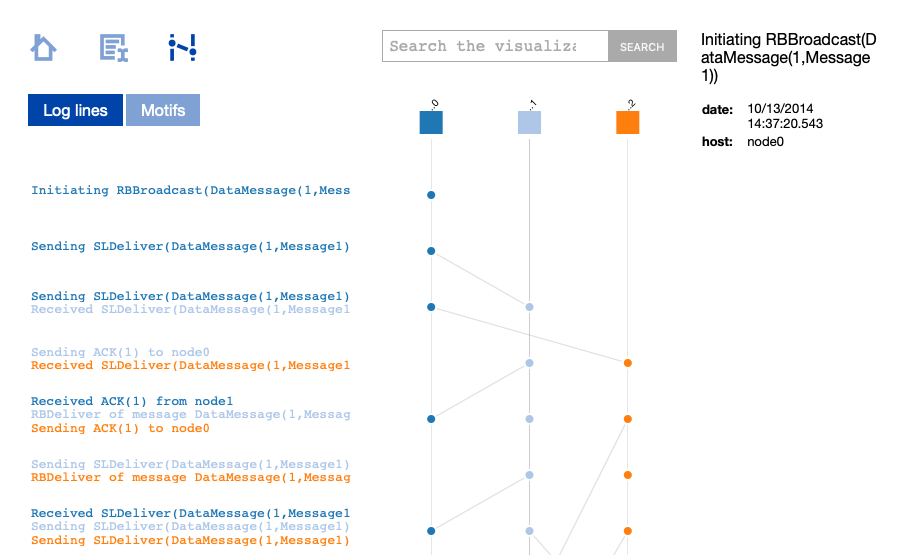
\includegraphics[scale=0.4]{ShiViz_Example.png} 
\centering
\end{figure}

\paragraph{Simulation Suite for Distributed Software}

The primary software that was used in this project is the SSDA created by students at the University of Northern British Columbia.  This software gives users the ability to design a distributed system and test that system without having to pay the huge costs of buying all the necessary hardware \cite{SSDA}.  The tool provides many different pre-made topologies, like the hypercube shown in figure 2, that can be modified by the user, as well as the option to draw an entire network from scratch \cite{SSDA}.  
\begin{figure}[t!!]
\caption{SSDA user interface \cite{SSDA}}
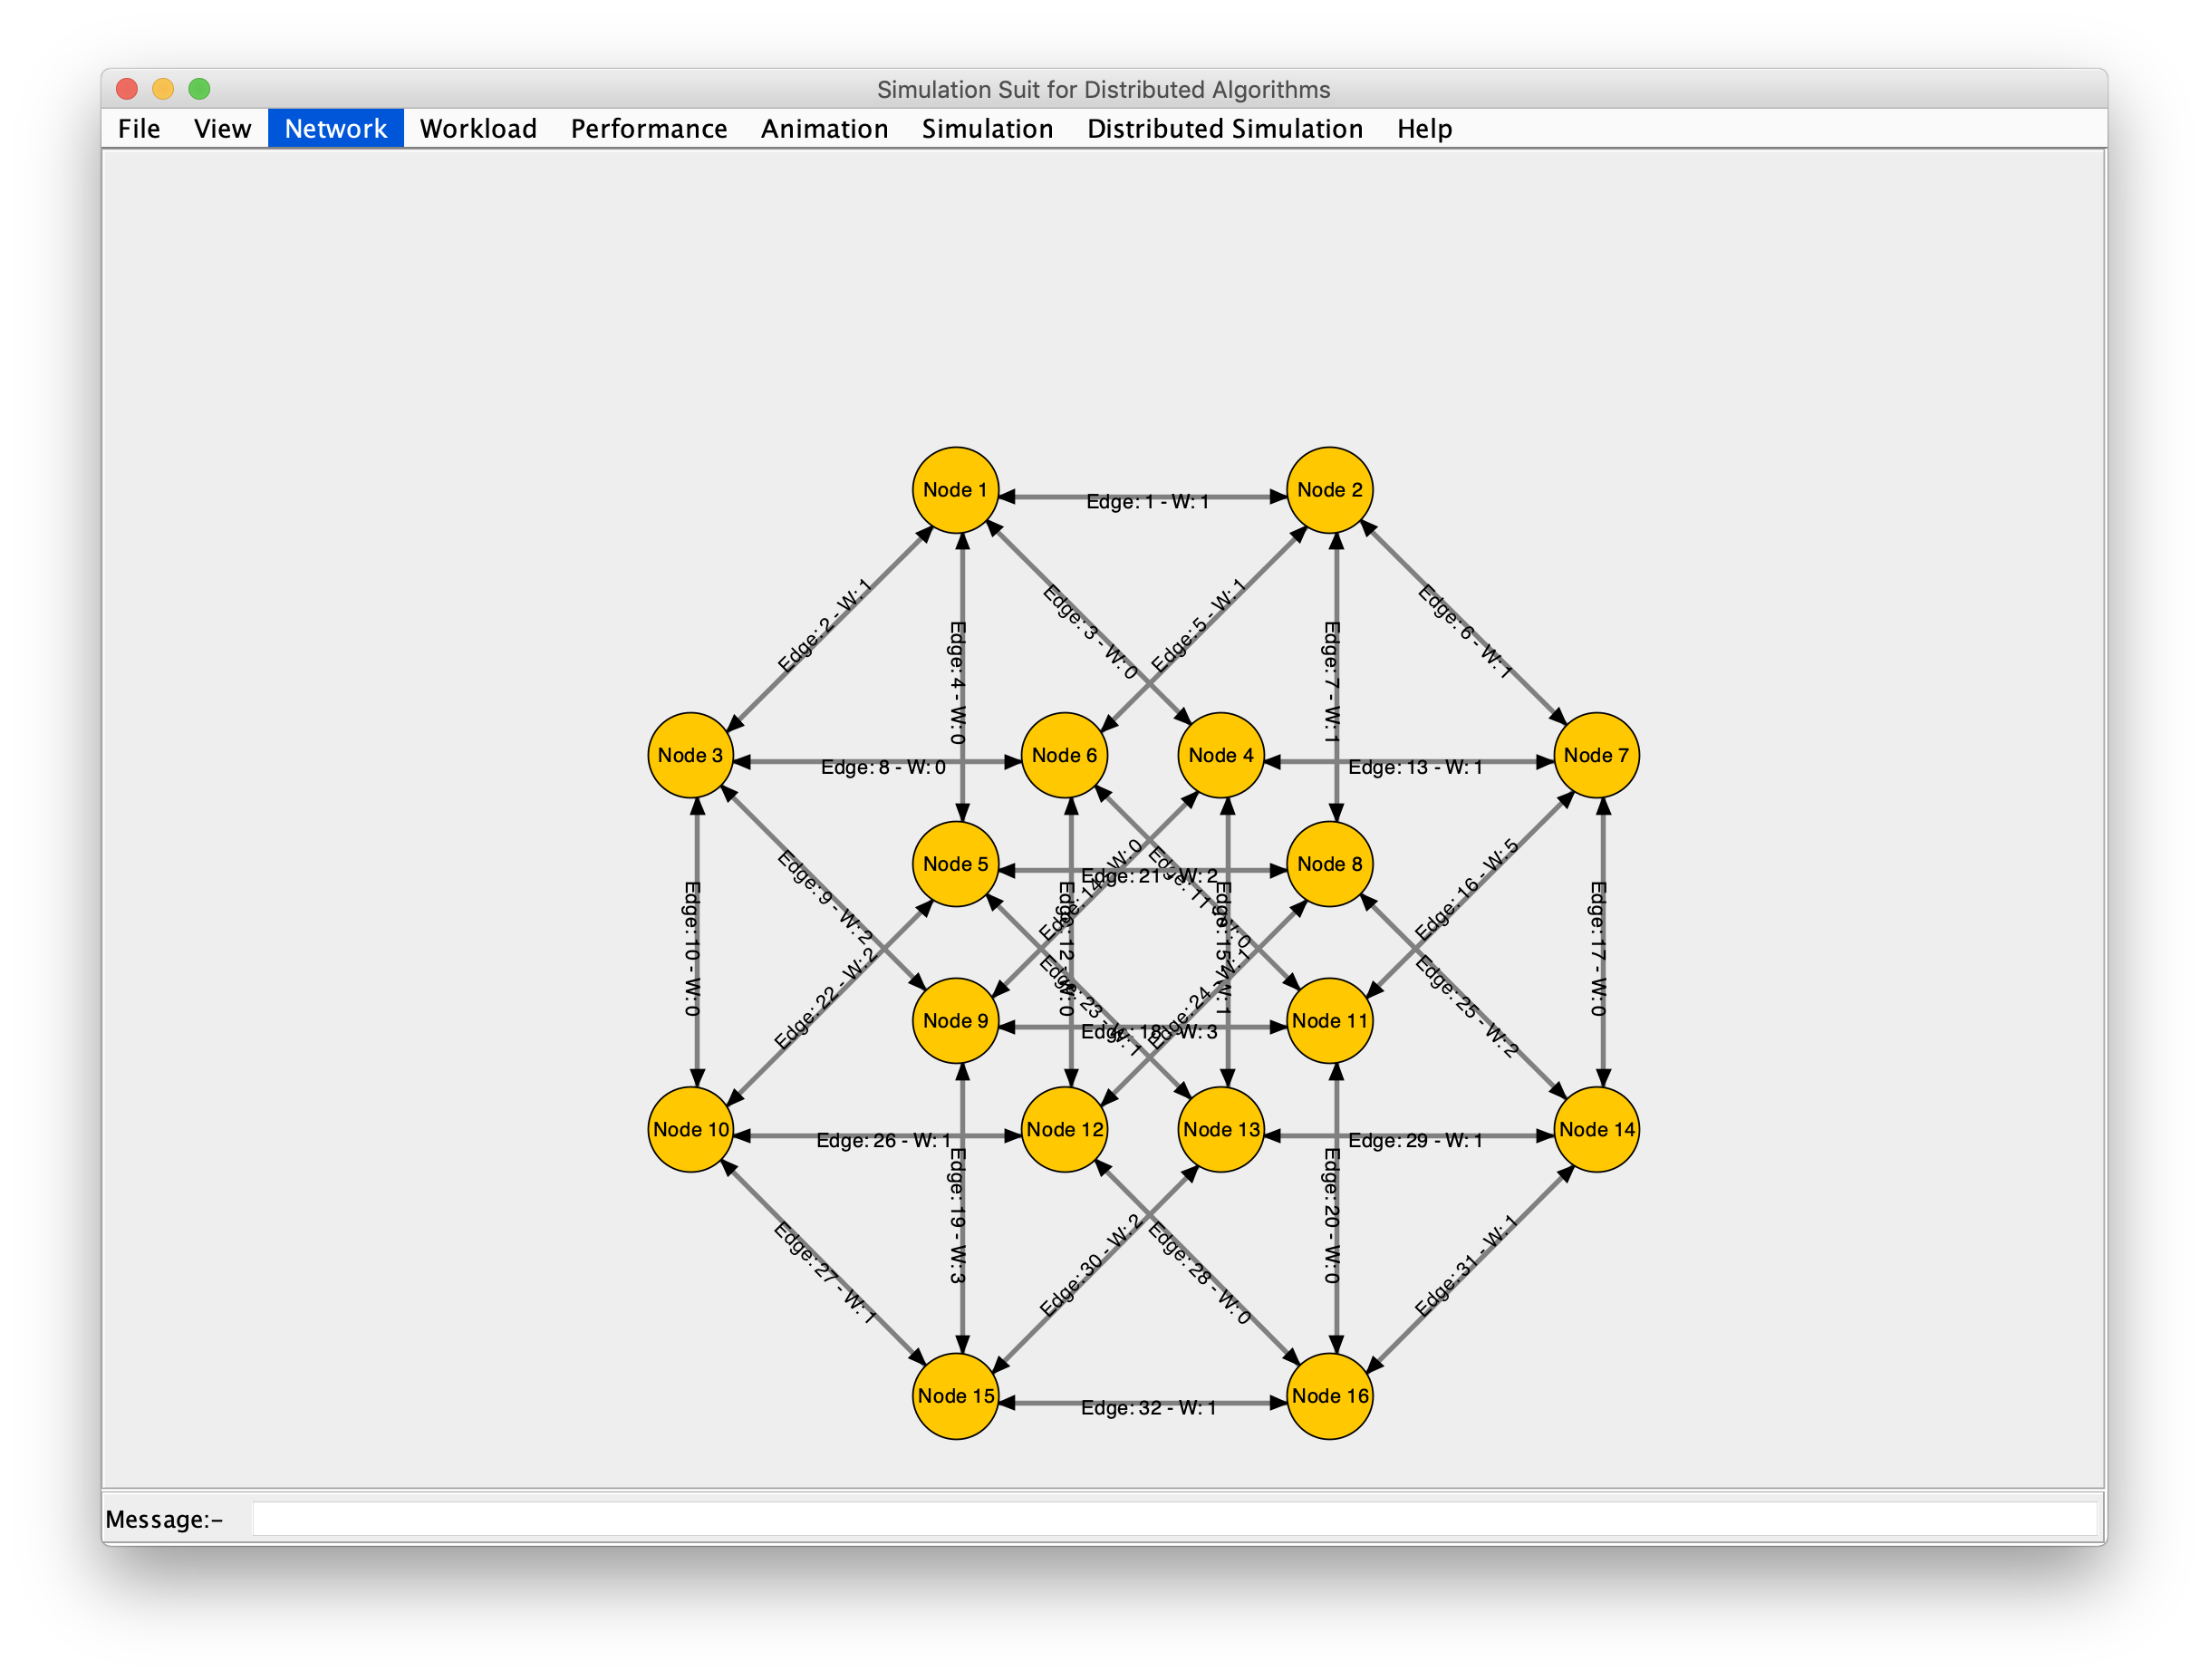
\includegraphics[scale=0.3]{SSDA_Example.png} 
\centering
\end{figure}The user creates nodes and then assigns connections between those nodes.  It is then possible to adjust the behaviour of each individual node as well as apply different settings to the entire network. There are other features of the app as well, like an animation that displays the flow of information from one node to another, as well as the ability to test and see the performance of a network \cite{SSDA}.  Networks can be saved and imported into the program as well.  SSDA offers users with many powerful tools to create and test virtual distributed systems.

\paragraph{Benefits of Integration}

Both of these softwares provide users with tools to visualize different aspects of distributed systems.  These tools, when combined, give users an even wider array of resources with which to learn about distributed systems.  By enabling the use of ShiViz's logs, users are able to see exactly where the flow of information between different nodes is.  It adds a more in depth layer of information that allows the SSDA to have more applications for a wider user base.

\paragraph{Changes Made}

There are no changes made to the ShiViz software and libraries, but there are a number of small changes to the SSDA.  The first additions made were adding the ShiViz vector clock library to the project.  After that the JVec class that was provided by ShiViz was incorporated into the SSDA.  To do that, a JVec object was created for each node and would record every time that a message is sent or received by that node. 
\begin{lstlisting}
//initializing the JVec object for a node
nodeObject.vcInfo = new JVec("Node" + nodeObject.getNodeId(), "LogFiles/Node" + nodeObject.getNodeId() + "LogFile");
\end{lstlisting}
This is called in the simulation class in the library package.  It is used after each node is created, giving that node the ability to generate it's part of the log for ShiViz.
\begin{lstlisting}
//sending a message in the send() method
encodedMsg = node.getVCInfo().prepareSend("Node " + getNodeId() + ": Sending Message: " + message.getContent(), message.getContent().getBytes());
//receiving a message in the receive method()
node.getVCInfo().unpackReceive("Node " + getNodeId() + ": Receiving Message: " + messageRecieved.getContent() + ", from node " + messageRecieved.getFinalSender(), encodedMsg);
\end{lstlisting}
These two lines are the ones that handle the sending and receiving of messages between nodes.  They were both added to the algorithm class in the library package.  The algorithm class is used by each node to send and receive messages in a variety of different ways.  The JVec library takes that information and converts it into a format that ShiViz can understand.  Once each node was being tracked by a JVec object, the GUI elements were changed to allow users to create ShiViz logs from within the SSDA.  Finally, a package was added to the project that takes all of the individual nodes' logs and condenses them into one that included the regular expressions needed by the ShiViz software.  This final step enabled 

\paragraph{How to Use the Modified Software}

In order for a user to create a ShiViz compatible log from within the SSDA, they simply need to click the box labeled "Generate ShiViz Log" on the Simulation page of the SSDA.  After setting up a simulation, it can be run by pressing the "Simulate" button.  This will create a Log file in the "LogFiles" folder in the same directory as the SSDA.  In order for the user to see ShiViz's visualization of the log file, they must open ShiViz in a browser.  By clicking the "Open ShiViz" button in the simulation screen of the SSDA, ShiViz will open.  Once there, clicking the "Try out ShiViz" button will bring them to a screen that will ask for a file (figure 3).
\begin{figure}[t!]
\caption{SSDA simulation panel \cite{SSDA}}
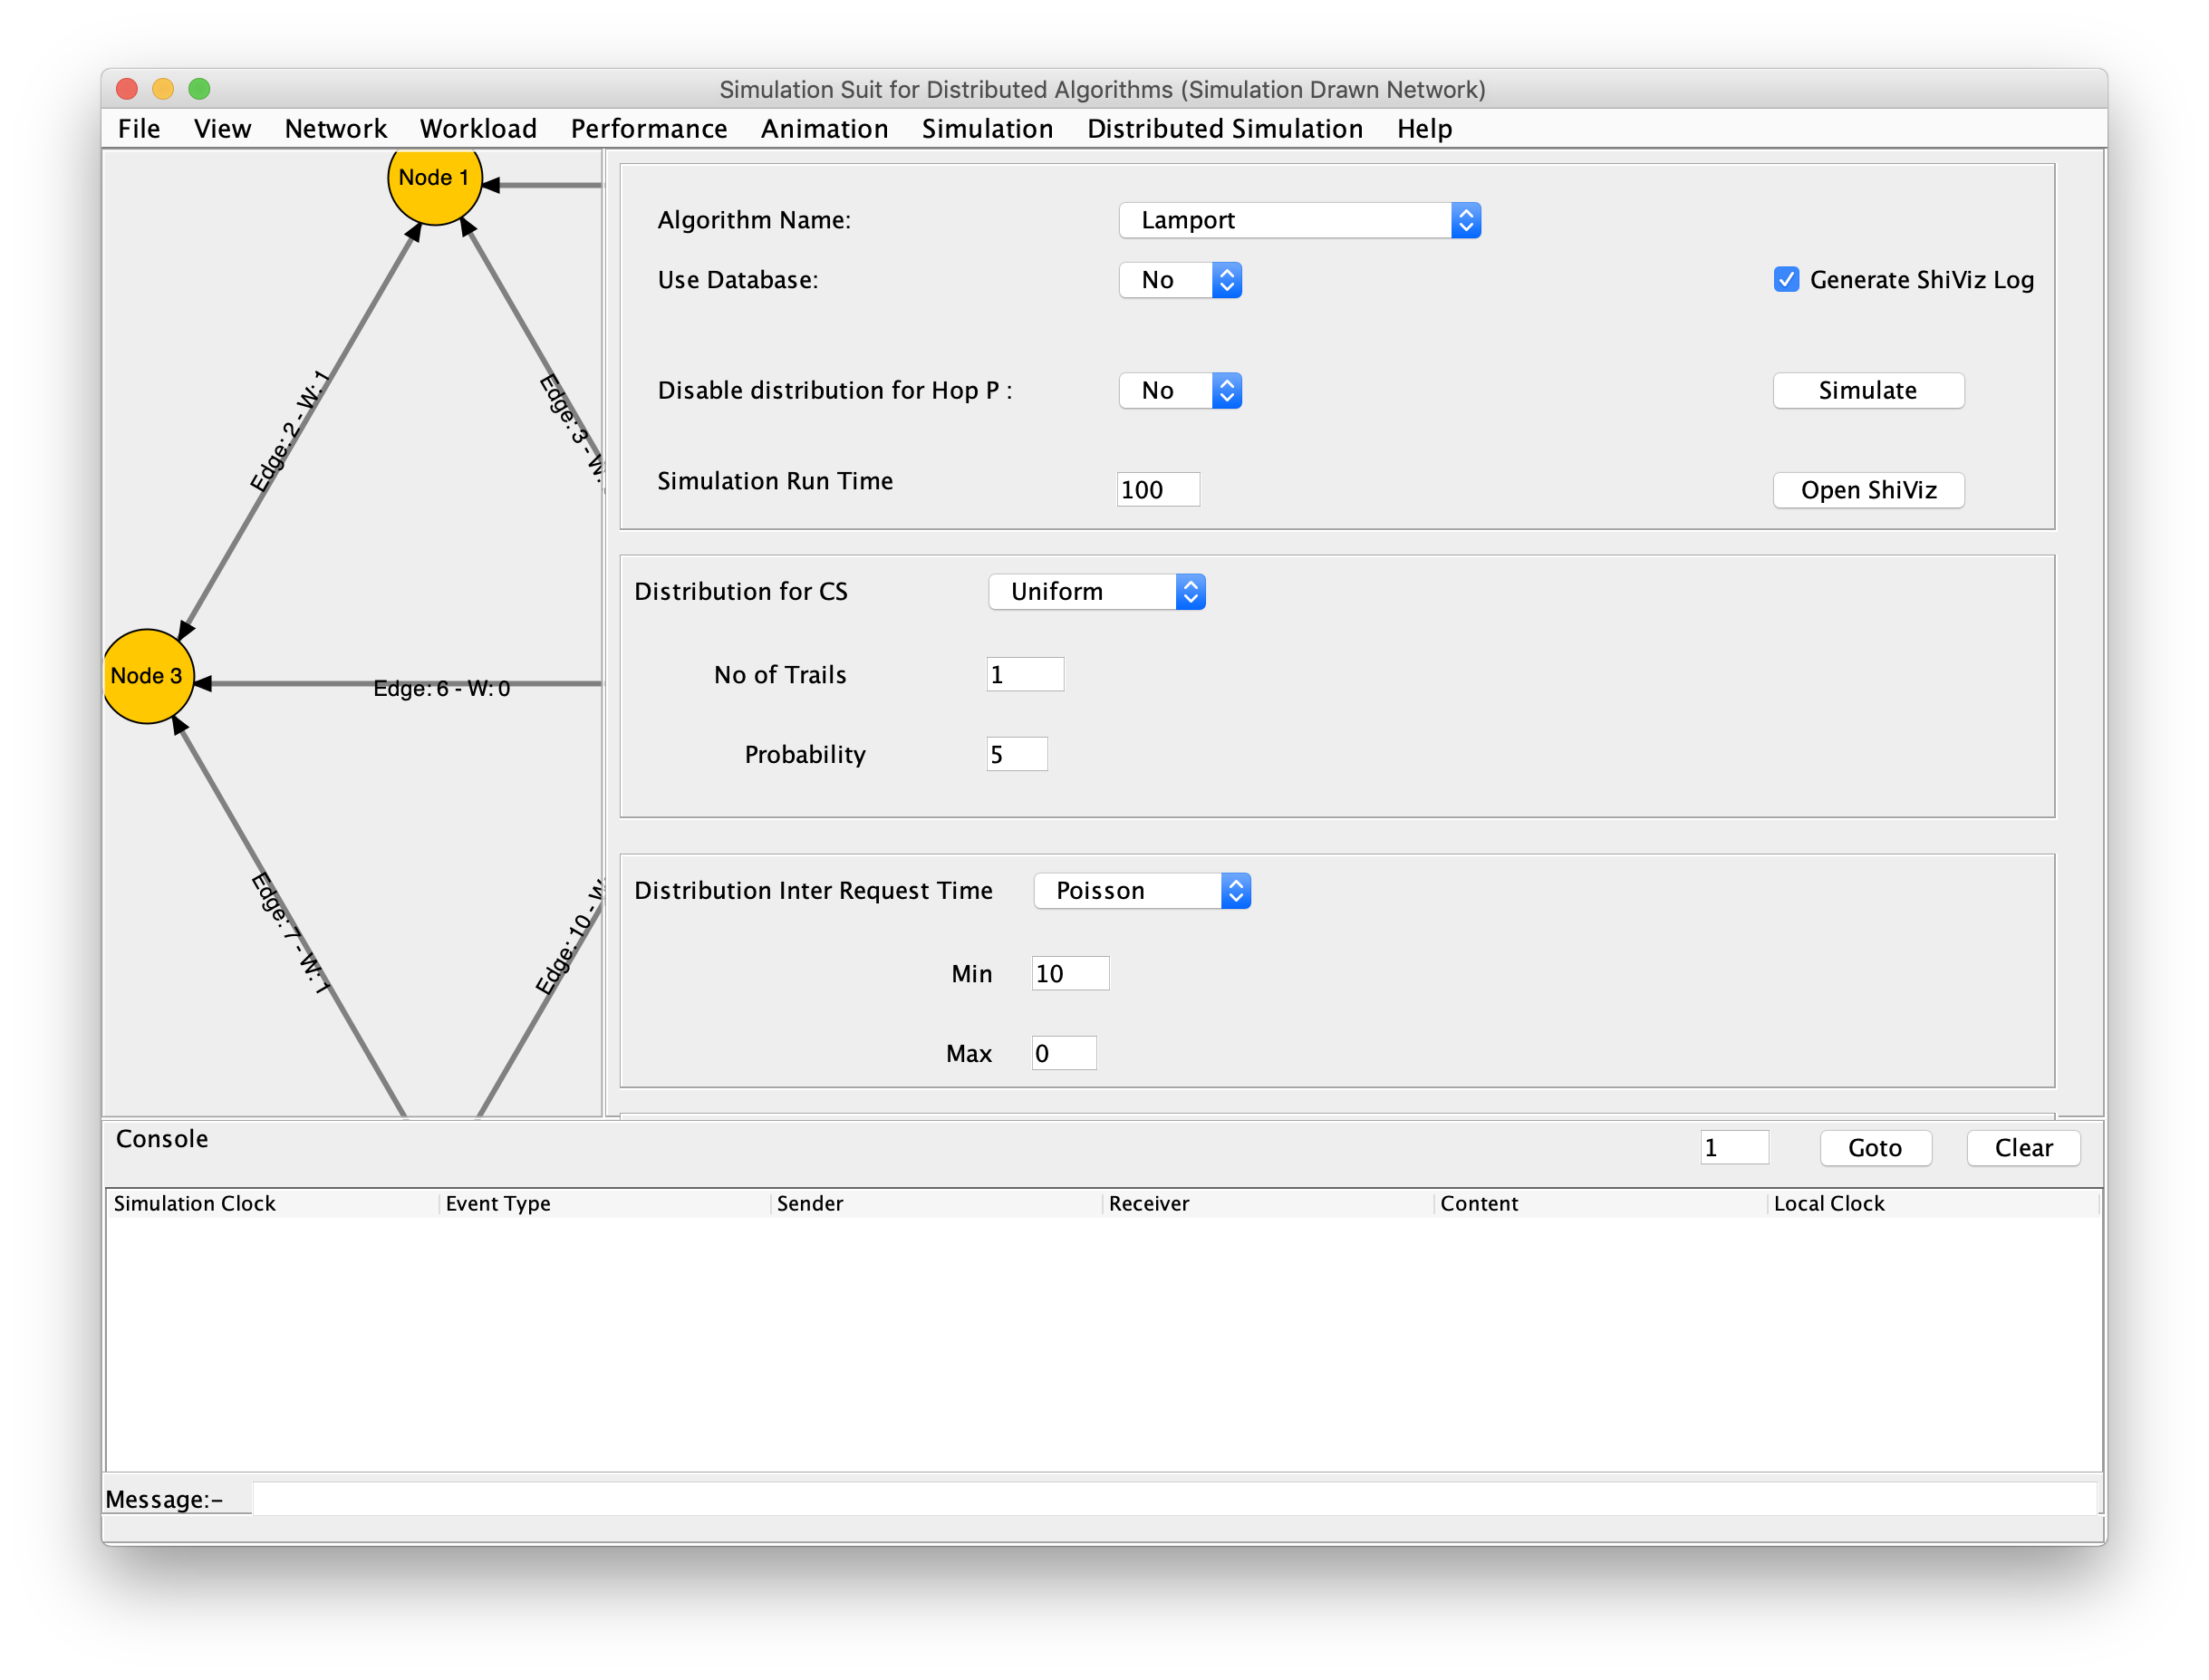
\includegraphics[scale=0.3]{SSDA_Sim_Window.png} 
\centering
\end{figure}
The appropriate file can be found in the LogFiles folder where the log was originally created.  The last step is to click "Visualize" and ShiViz will create a visualization of the selected log (figure 4).
\begin{figure}[t!]
\caption{ShiViz file manipulator \cite{ShiViz}}
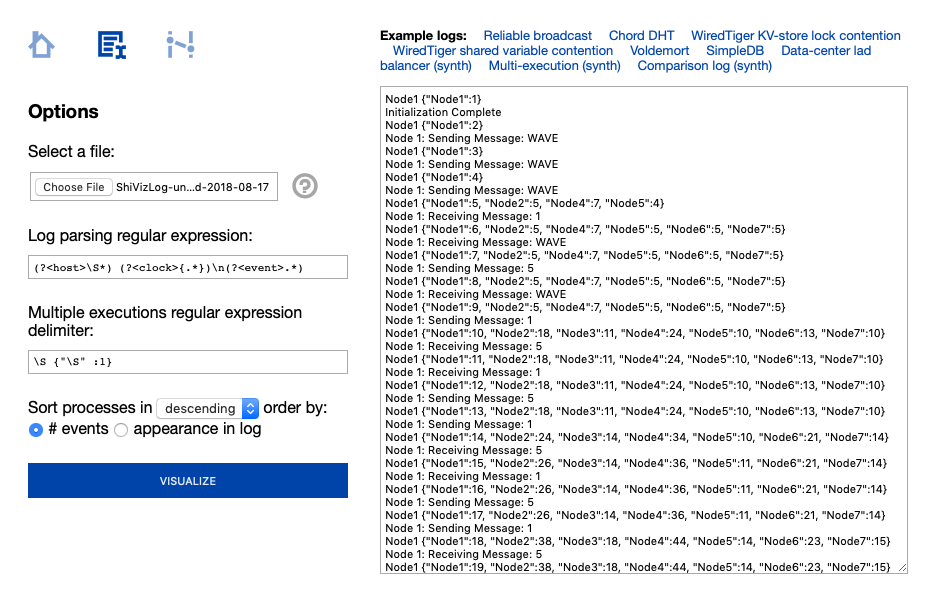
\includegraphics[scale=0.5]{ShiViz_File.png} 
\centering
\end{figure}

\paragraph{Challenges Faced}

There were many challenges faced while completing this project.  Much of the time early on was spent learning about the basics of distributed systems and what the two softwares could do.  It took some time to fully understand what was needed.  Once all of the research was complete, the next hurdle was understanding where to properly integrate the ShiViz vector clock library with the UNBC software.  Creating the logs and recording each sent message was relatively straightforward, but properly recording the received messages proved to be quite the task.  This took longer than anything else and required much more research into what exactly was happening in the library.  Eventually, after much time and frustration, the solution was found by using the encoding provided upon message creation and decoding the message at the receiver's end.  With that challenge complete, the remaining polish was not difficult.  Adding UI elements and consolidating all of the individual logs was simple File IO.

\paragraph{Conclusion}

Both the SSDA and ShiViz are powerful tools that can help people in many different distributed systems applications.  By combining the two, their usefulness has only grown.  In the future, there is potential for the SSDA to improve, with its distributed simulation feature already being a work in progress.  There is also an opportunity to expand upon the algorithms available for simulation.  On the other hand, ShiViz is already a completed product and there does not appear to be any more work planned for it\cite{ShiViz}.
\newpage
\bibliography{References}
\bibliographystyle{plain}
\end{document}   